\section{Control system design}

The path following control problem can be simplified to a course control problem, if:

\begin{itemize}

	\item The waypoints are adequately close to each other, or the path is populated with subwaypoints placed adequately close to each other
	\item The waypoints are marked as visited, if the ship approaches them to a certain nonzero distance

\end{itemize}

Relying on the conditions above in not always possible, therefore the controller has been extended with position-control. If the feedback of the position error is zero, the resulting controller is identical to the simple heading controller.

\subsection{The combined control problem}

The following control system has been developed for the Rudder ship type, in order to parallelize my efforts with the RobonAUT controller development, which is generally the same control problem, if the simplified system dynamics are used.

The path following problem can be traced back to a balancing problem, specifically where the ball must be kept in the center of a seesaw: [illusztrációk]
We know the dynamic behavior of the system:

$\dot{d} = g-$
$Delta_dot$

So the control problem of the boat (or car) following the path (or line) is in a narrower sense the same as leveling the seesaw with the ball in the center. [labjegyzet: in a narrower sense: this statement is only valid until the ball hits the end of the seesaw (or falls out) and the divergence of the car ($\delta$) is in $[-pi/2, pi/2]$]

A wide range of controllers has been evaluated in order to determine the best approach to solving this control system.

\subsection{Requirements of control}

\subsection{Controllers for deterministic systems}

Using the linearized state transition matrices the transfer function of the system can be formulated using:

\begin{align}
	H(s) = C*(sI - A)^{-1}B + D
\end{align}

The resulting system is a 2nd order integrator, which isn’t a surprise, if we consider the linearized output d based on the input $\Phi$

Using this transfer function a PID steering controller can be designed to control the system.

\begin{figure}[H]
	\centering
	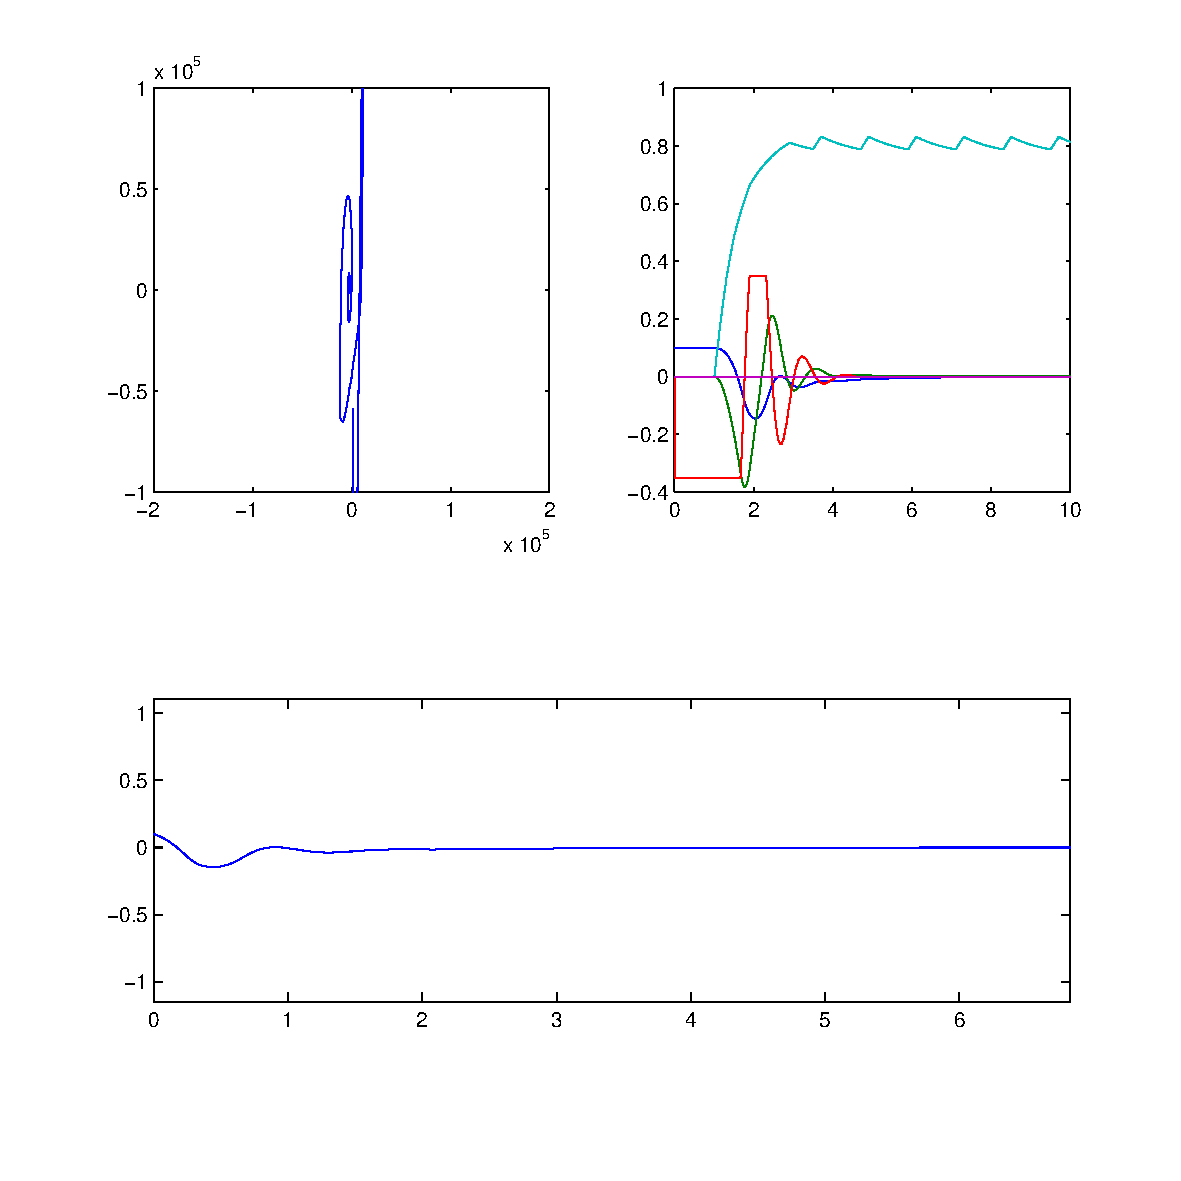
\includegraphics[width=0.8\textwidth]{img2/PI01}
	\caption{}
	\label{}
\end{figure}

The system response quality is generally low but adequate, but the serious problems arise when the system starts with larger initial conditions that are significantly different from the approximation point.

\begin{figure}[H]
	\centering
	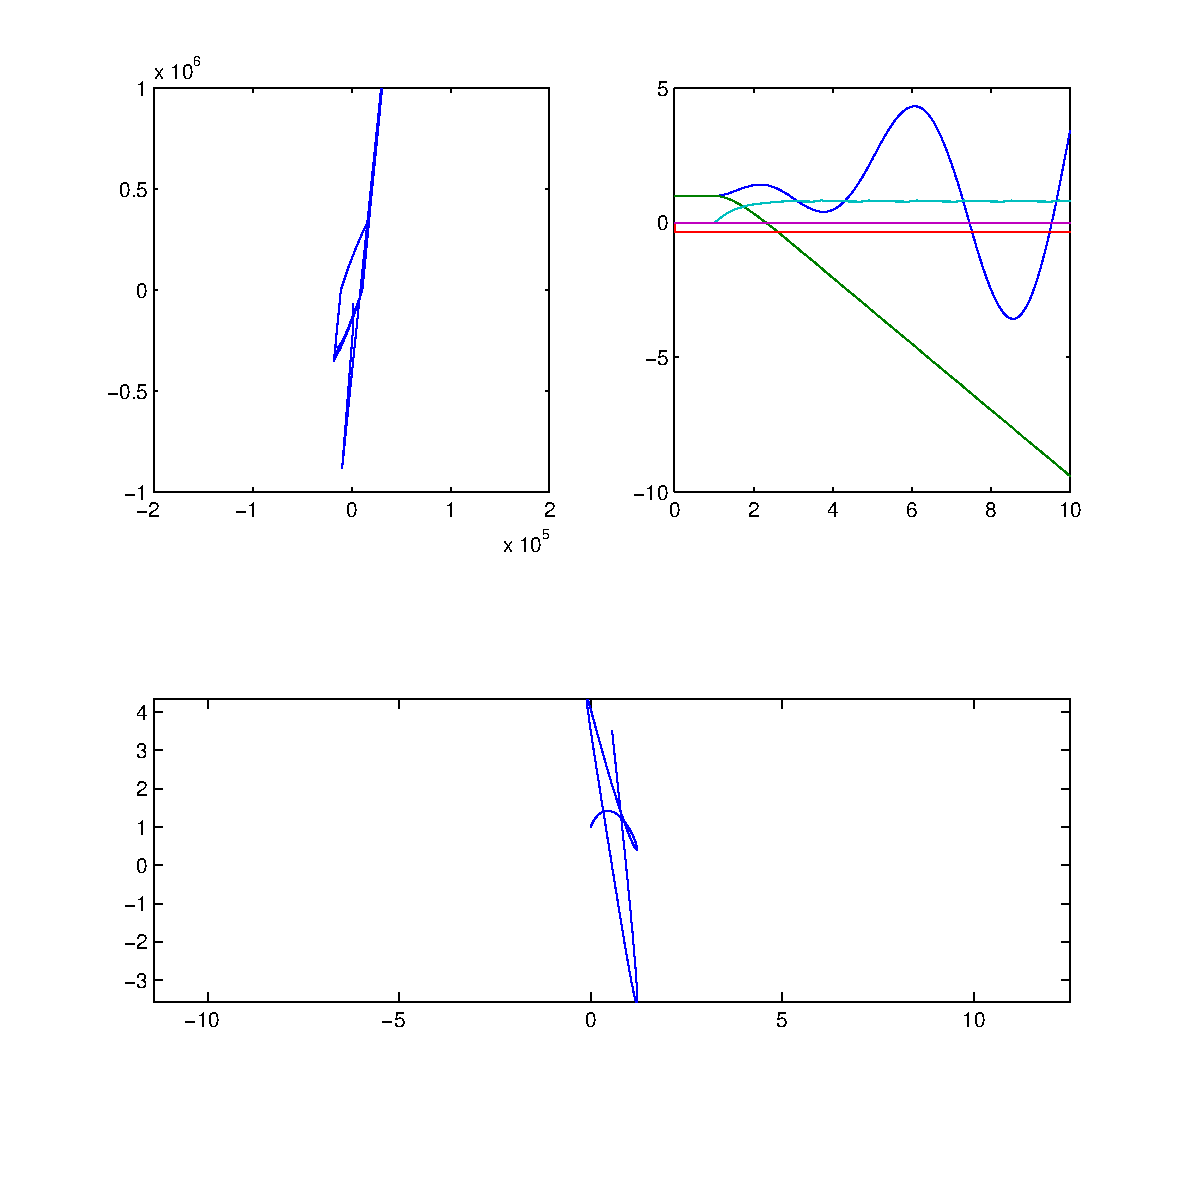
\includegraphics[width=0.8\textwidth]{img2/PI11}
	\caption{}
	\label{}
\end{figure}

The conclusion is that it’s unwise to use the pole cancelation based PID control to regulate an unstable, significantly nonlinear system. The robustness of the PID is generally low, and the system response is slow. The resulting control system is slow and unreliable.

\subsection{State-feedback controller}
In order to enhance the system response, a full state feedback controller can be computed using the same linearized system. The pole placement method allows the efficient control of unstable system, but how does it’s robustness fair against the nonlinearity of the system?

\begin{figure}[H]
	\centering
	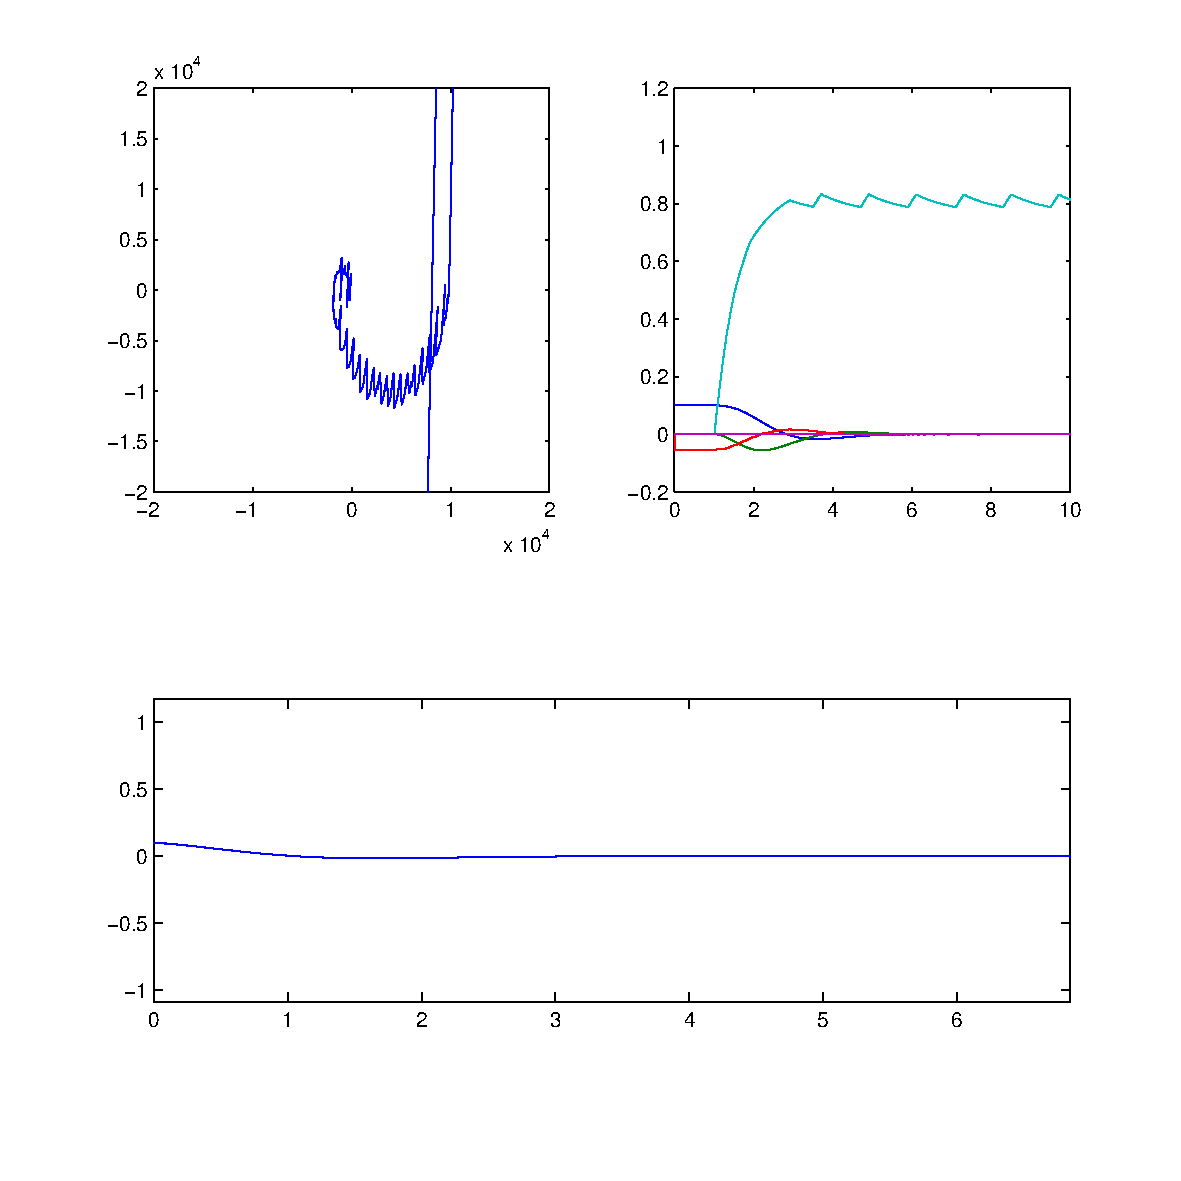
\includegraphics[width=0.8\textwidth]{img2/Lin01}
	\caption{The physical layout of the system}
	\label{fig:PhysicalLayout}
\end{figure}

The response speed is much better than the respone of the PID controller, but it contains an overshoot, which is the result of the nonlinearities. Here however the pole placement method placed the poles to imperfect locations, instead of entirely missing a pole with a zero.

\begin{figure}[H]
	\centering
	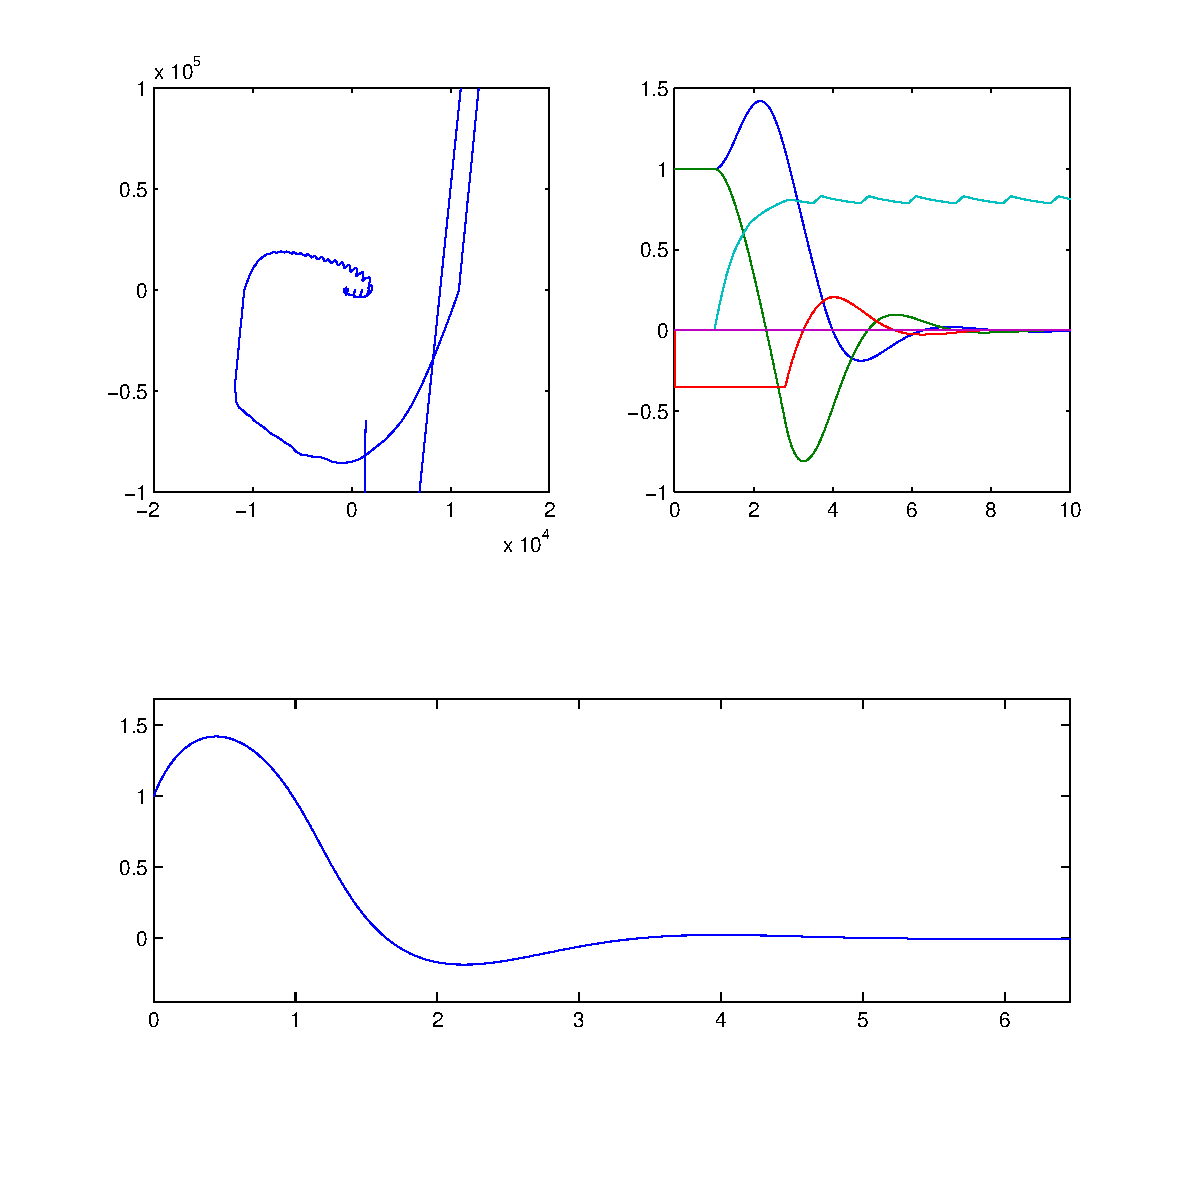
\includegraphics[width=0.8\textwidth]{img2/Lin11}
	\caption{The physical layout of the system}
	\label{fig:PhysicalLayout}
\end{figure}

As expected, the simulation result of the larger initial conditions is overshoot and oscillation, but the system will quickly settle. Of course this is not good enough yet, because the system is balancing on the edge of instability, and the effects of nonlinear sensors and measurement limitations will have additional negative effects that can cause instability.

Conclusion: the full state feedback linear controller can control the system in most cases, but is unfit to control a mission-critical system, because it has inadequate robustness and reliability.

\subsection{Hybrid switching state-feedback controller}
The instability of the linearized state-feedback controller at high Delta can be corrected by using a Hybrid controller.
the Hybrid is the bridge between linear and nonlinear control systems. The controller contains multiple state feedback controller implementations of the same system, linearized around different approximation points. The control task consists of finding the best controller for the current states, and controlling the system as a locally linear system.

For small initial conditions the Hybrid behaves exactly like a regular linear full state feedback controller.

\begin{figure}[H]
	\centering
	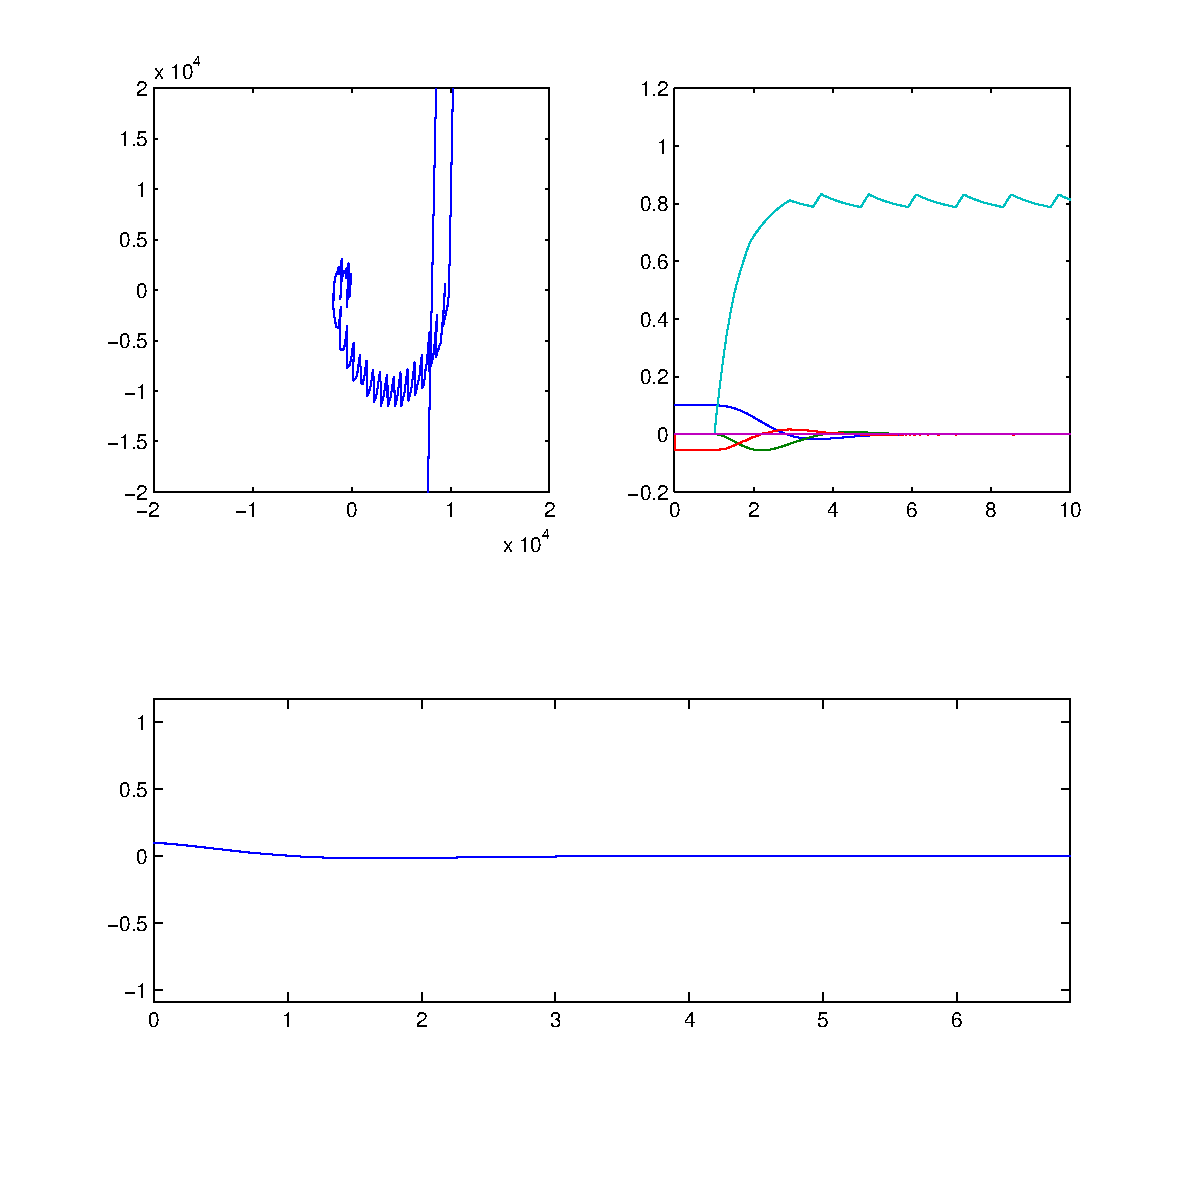
\includegraphics[width=0.8\textwidth]{img2/Hyb01}
	\caption{}
	\label{}
\end{figure}

For large initial conditions however, a different controller implementation is selected to increase the response quality. In this case however the system reaction involves only small nonlinearities, therefore a slight decrease in settling time can be observed, but nothing major. As the $\Phi_{max}$ is increased, so does the nonlinearity of the control signal, and the more the response quality is increased by the hybrid controller compared to the linear.

\begin{figure}[H]
	\centering
	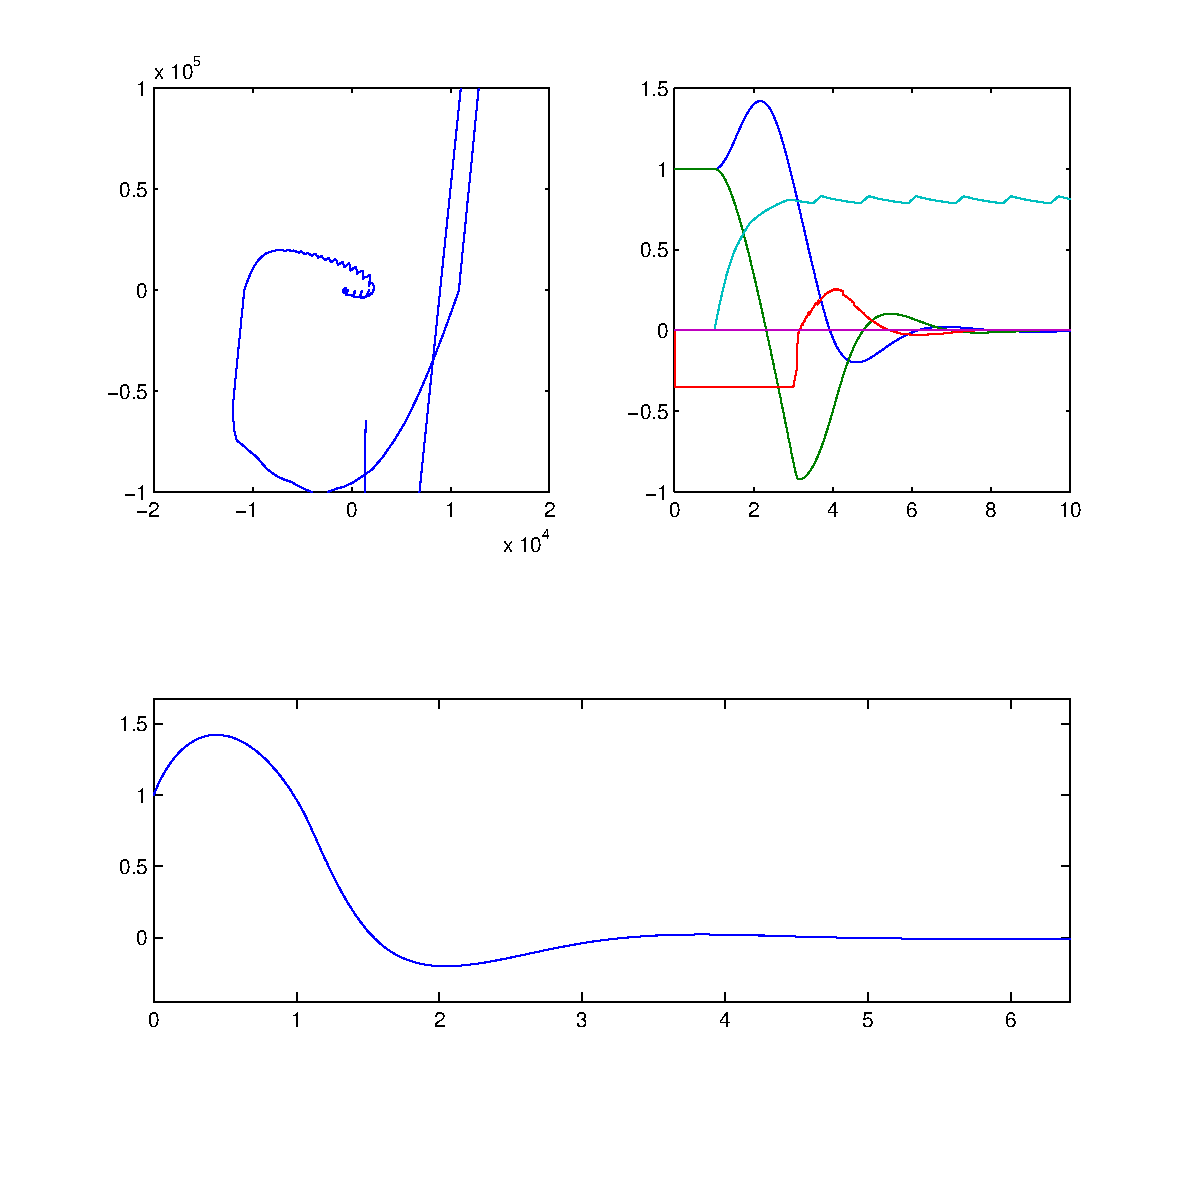
\includegraphics[width=0.8\textwidth]{img2/Hyb11}
	\caption{}
	\label{}
\end{figure}

The Hybrid controller has serious dangers and disadvantages however. If the control switching is not implemented correctly, it is possible to destabilize a stable system, and trigger the divergence of the states.
Additional disadvantages include the unwanted and unpredictable system responses if a controller switch occurs. This problem can be reduced by controlling the change of the control signal, instead changing the control signal directly, therefore the jumps in the control signal can be eliminated.
Another disadvantage is the possible necessity of having a large number of controller implementations. For example, linearizing around 3 state variables with a definition of 10 linearizations each results in 1000 separate controller implementations.

If having a large number of control implementations is not a problem, the process can be automated using the symbolic toolbox of MATLAB (or any other similar software) if the correct nonlinear state-transition functions are know.
The symbolic toolbox allows the automated formulation of the Jacobi matrices and the software can compute the linearized implementations cyclikally, then store them in a lookup table. 

\subsection{Fuzzy controller}
Though linearizing around many approximation points can result in a relatively smooth switching experience, the number of required controllers can quickly become unreasonably high. The fuzzy controllers address these problems and provide a solution for smooth switching and low number of controllers. Additional advantage of the fuzzy controller is the Fuzzy Control Language, which is the de-facto standard Domain Specific Language for developing fuzzy logic and controllers. The use of FCL helps to understand and design the switching methods which is an important part of the Hybrid controller design.

The Fuzzy controller has an important property that differenciates it from the rest of the controllers evaluated here: the formulation of the control system is based on “liquid” facts, instead of solid data. This results in a less-optimal control, but can ensure stability for systems with unknown dynamics. The fuzzy controller is expected to produce a system response of lesser quality, however it’ll have an important role in controlling the more complex, only partially known ship dynamics presented earlier.

Unfortunately there was no time to finish the testing of the Fuzzy controller, therefore the results will be included in a later version of the document. 

\subsection{State Ordinance Controller}
The system response can be enhanced further using unconventional controllers. This “State Ordinance Controller” (OC) couldn’t be any more unconventional, because it’s the result of my early ignorant implementation of a sliding mode controller, but it can provide surprisingly good system responses and boasts a very simple mathematical background and implementation.

The essence of the OC is to determine a priority order of state variables and control the individual states separately by specifying spaces and surfaces. By forcing the state variables into the spaces and onto the surfaces, arbitrary system response can be achieved (of course the physical limitations apply here as well).

The example system is the steering control of the car. The divergence ($\delta$) is forced onto a surface function of distance (d) by controlling $\Phi$. If $\Phi$ is controlled correctly, $\delta$ will stay on the surface. If the surface has been defined in a way that if $\delta$ is on the surface then
$$
\dot{d} = f(x)
$$
function is negative-definite, then d and $\delta$ will approach zero together.

[figure]

Considering the nonlinearities of the system

$$
max(|\dot{d}|) = v
$$

if $\delta = +-pi/2$. This generates the highest-priority natural space for $\delta$.

So $\delta$ is forced to onto the following final function:

[figure]

So a basic implementation of the control system could be:

\begin{align}
	\Phi = sgn(sat(d,[-\frac{\pi}{2};\frac{\pi}{2}]) - \delta) * \Phi_{max}
\end{align}

Of course the controller response would be a high-frequency switching of $\Phi$, resulting in Zeno's paradoxes, which is undesireable. So instead of the signum function another saturation function can be used with values between -1 and 1, with an additional permissible error ($\varepsilon$) parameter. The higher the permissible error, the lower the frequency of the chattering will become.

\begin{align}
	\Phi = \frac{sat(sat(d,[-\frac{\pi}{2}; \frac{\pi}{2}]) - \delta, [-1; 1])}{\varepsilon} * \Phi_{max}
\end{align}

Re resulting system response:

\begin{figure}[H]
	\centering
	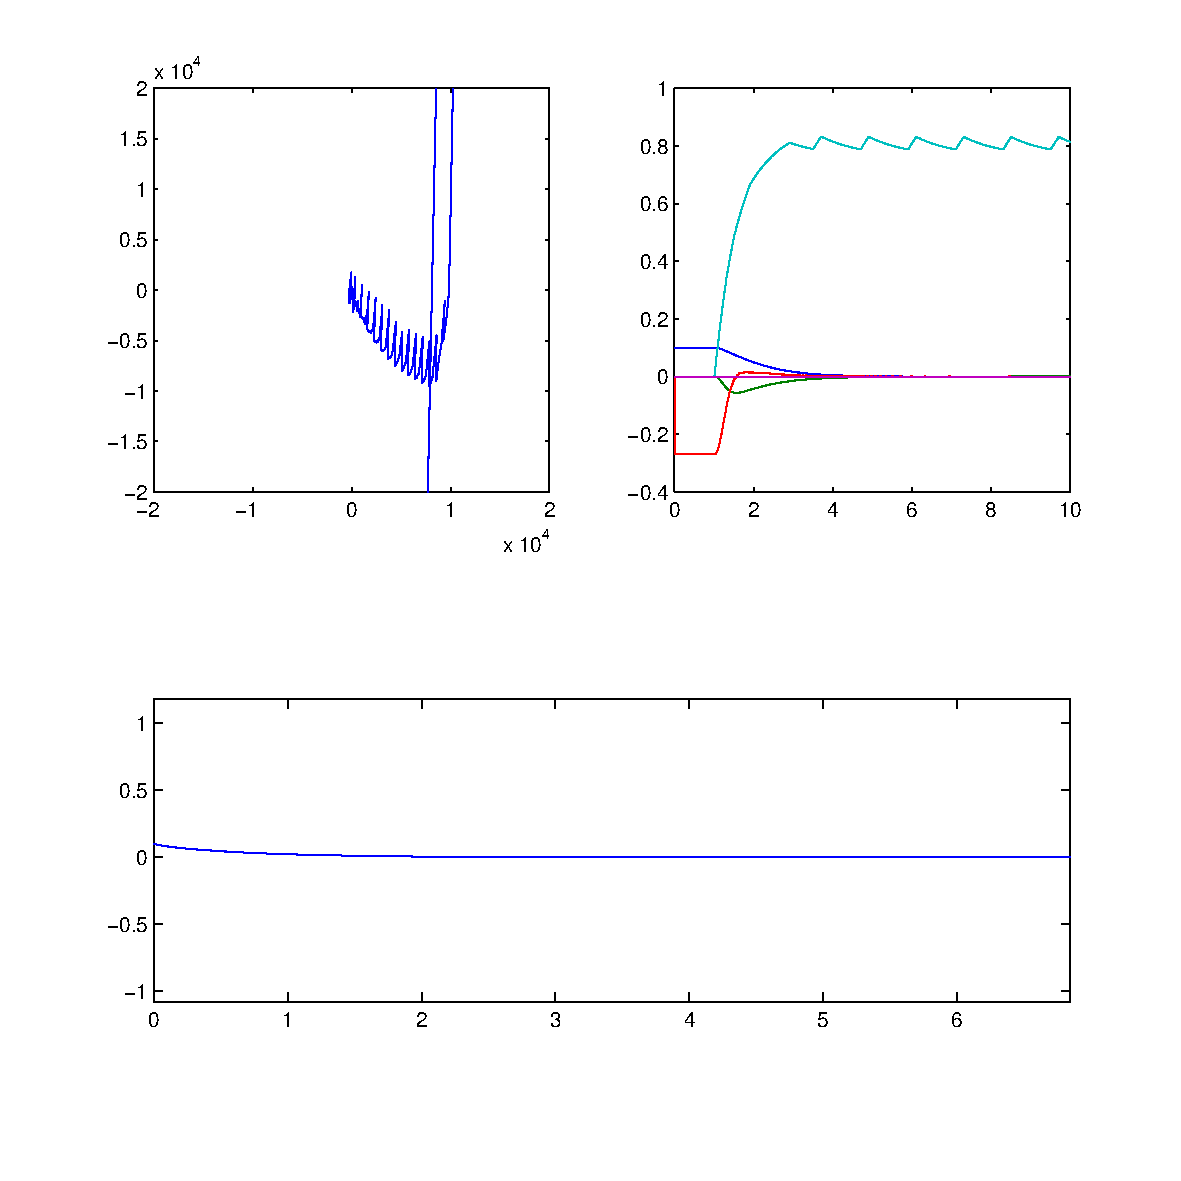
\includegraphics[width=0.8\textwidth]{img2/Ord01}
	\caption{}
	\label{}
\end{figure}

And the resulting system response fir large initial conditions:

\begin{figure}[H]
	\centering
	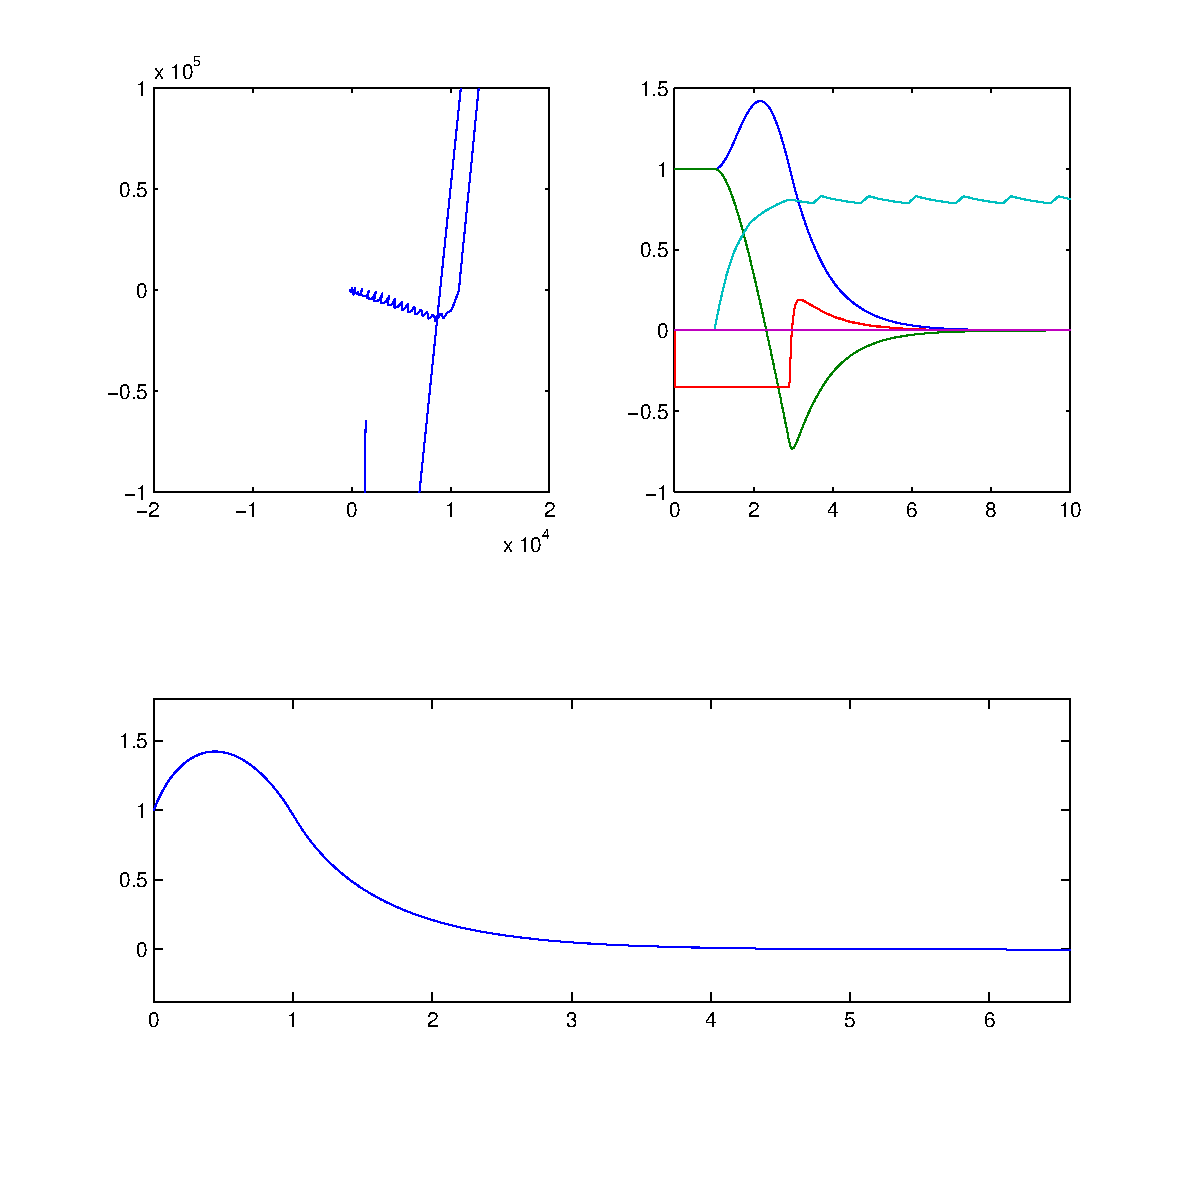
\includegraphics[width=0.8\textwidth]{img2/Ord11}
	\caption{}
	\label{}
\end{figure}

By changing the natural space of $\delta$, different trajectories can be achieved, like a shallower approach to the path:

[figure][figure]

Additional spaces or surfaces can be introduced, like the limitation of $\Phi$ based on the speed and the limitation of the acceleration based on $\Phi$ for a basic traction control.

The resulting control system excels in robustness and system response speed, but the order of prioritizing the state variables requires some intuition (general rules of thumb can be applied however).
The downsides are the virtually nonexistent documentation (excluding this document) and lack of mathematical background (yet).

The result is a robust and fast controller for any initial conditions and some system inaccuracies, and can be considered reliable because the controller can be formulated directly to the nonlinear system.

I consider this type of controller the bridge between fuzzy control and the Sliding Mode Controller.

\subsection{Sliding Mode Controller}

The Sliding Mode Controller is an ambivalent control method. It’s a very powerful tool to directly control nonlinear systems, but the formulation can be tricky.

“The common Lyapunov function is an elusive beast that you can almost never find.” [Magnus Egerstedt, Associate Chair for Research and External Affairs, Georgia Institute of Technology]

The central concept of the Sliding Mode Controller is to combine the deviations of the state variables from the reference input and unite them in the combined error function. Then use the Lyapunov function of the dynamical system to prove that there exists a controller that the trajectory of the combined error will hit a surface, starting from every possible initial condition, and then it will move along the surface to reach zero.

In practice a Lyapunov candidate function can be determined, then design the controller based on the combined error function.
Formal proving that such a controller exists is very hard, but in the current control case general considerations can lead to the same conclusion: it does. If $\Phi ~= 0$ then the system is stable (not asymptotically stable, but stable). Therefore a sliding surface can be determined for the combined error function.

The system response is quick and lacks the overshoot

\begin{figure}[H]
	\centering
	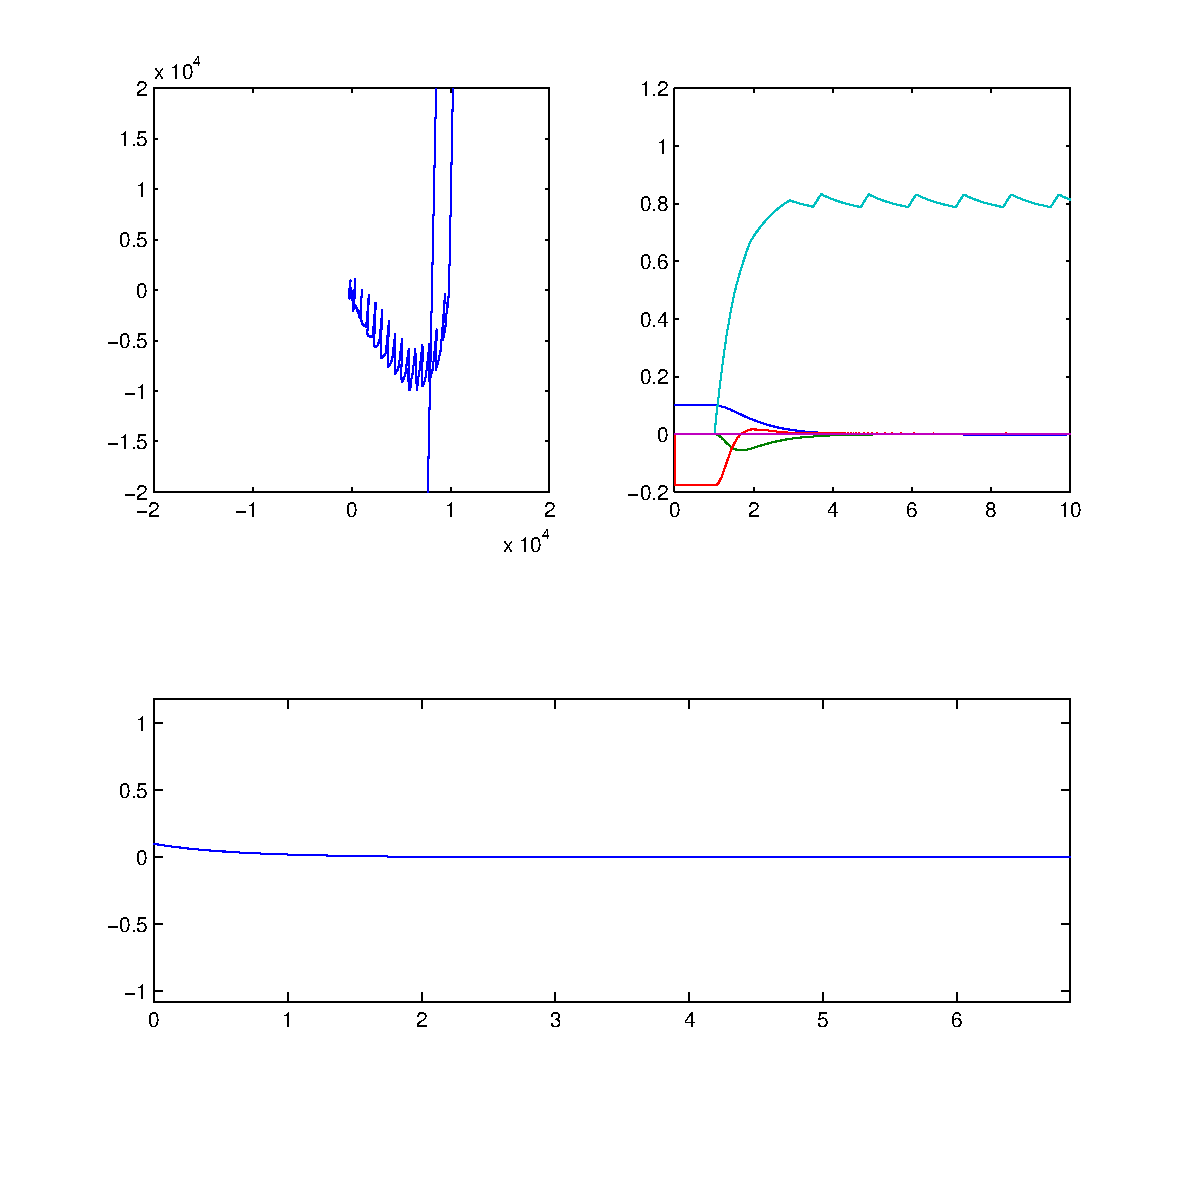
\includegraphics[width=0.8\textwidth]{img2/Sli01}
	\caption{The physical layout of the system}
	\label{fig:PhysicalLayout}
\end{figure}

And very reliable for larger initial conditions as well.

\begin{figure}[H]
	\centering
	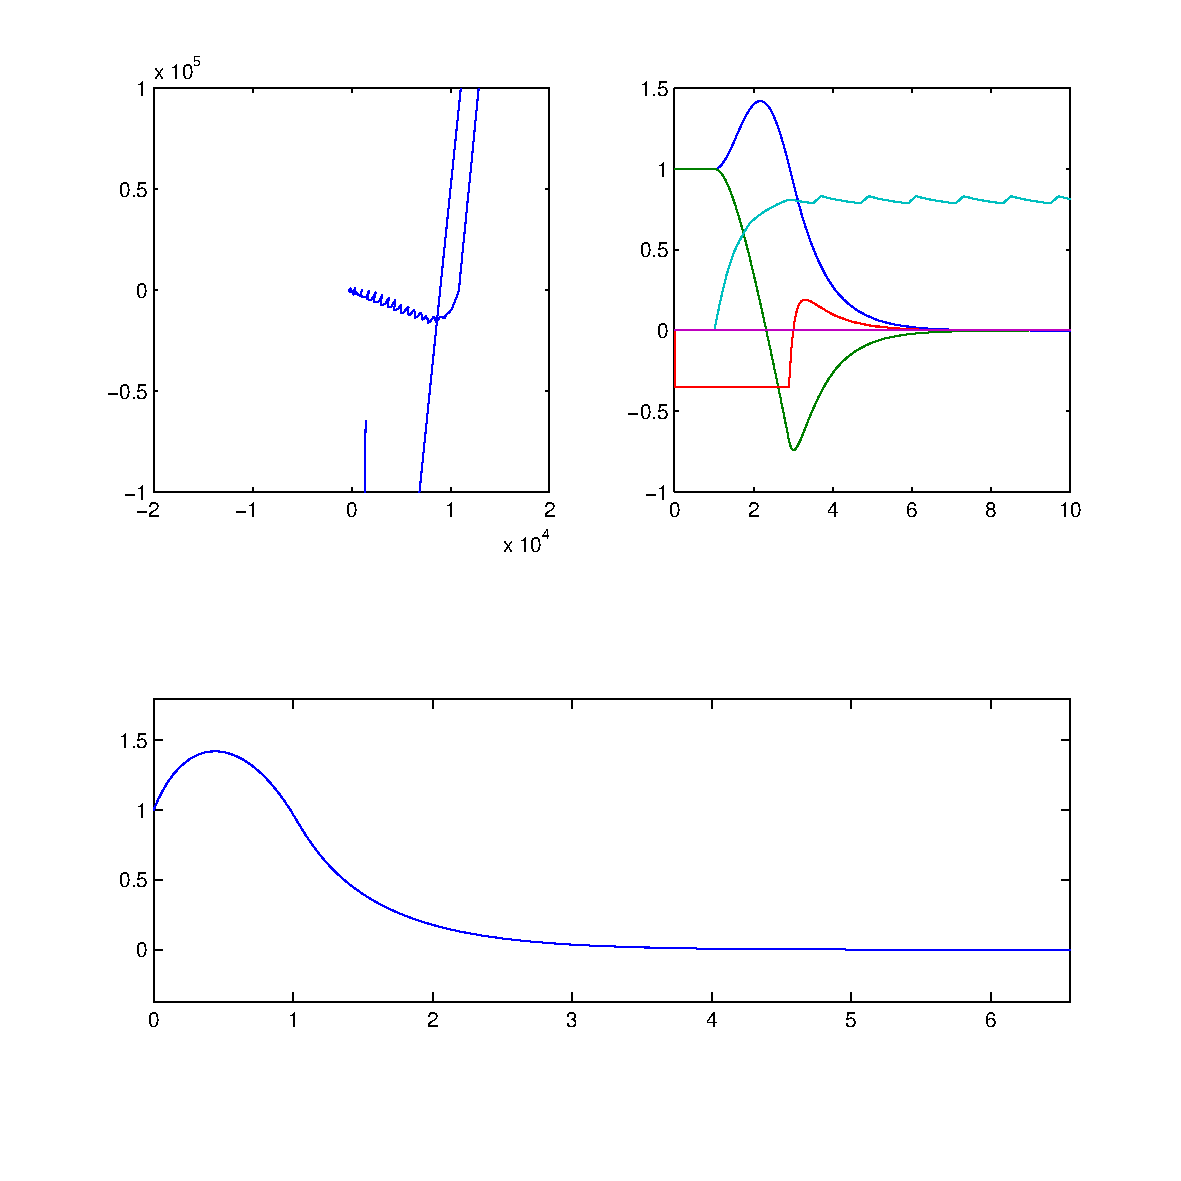
\includegraphics[width=0.8\textwidth]{img2/Sli11}
	\caption{The physical layout of the system}
	\label{fig:PhysicalLayout}
\end{figure}

\subsection{Model predictive control}

The model predictive control was not evaluated, because the control problem at hand allows quick data acquisition and has virtually zero time-delays. The real strength of model-based control is to predict the states and outputs of a complex system based on numerous inputs, if relatively large time delays are present. The model-based control is ineffective at small scale operations, because it’s very CPU-heavy, and it’s prediction capabilities are useless with a fast system responses.

Alas, a precise model of a large scale ship includes several underlying states with delayed effects, thus calling for a model predictive control, because a single tiny overshoot in the orientation control of a container-transport can be measured in kilograms of fuel.

\subsection{Comparsion of results}

The evaluation results of the controller types are depicted in the following diagram:

\begin{figure}[H]
	\centering
	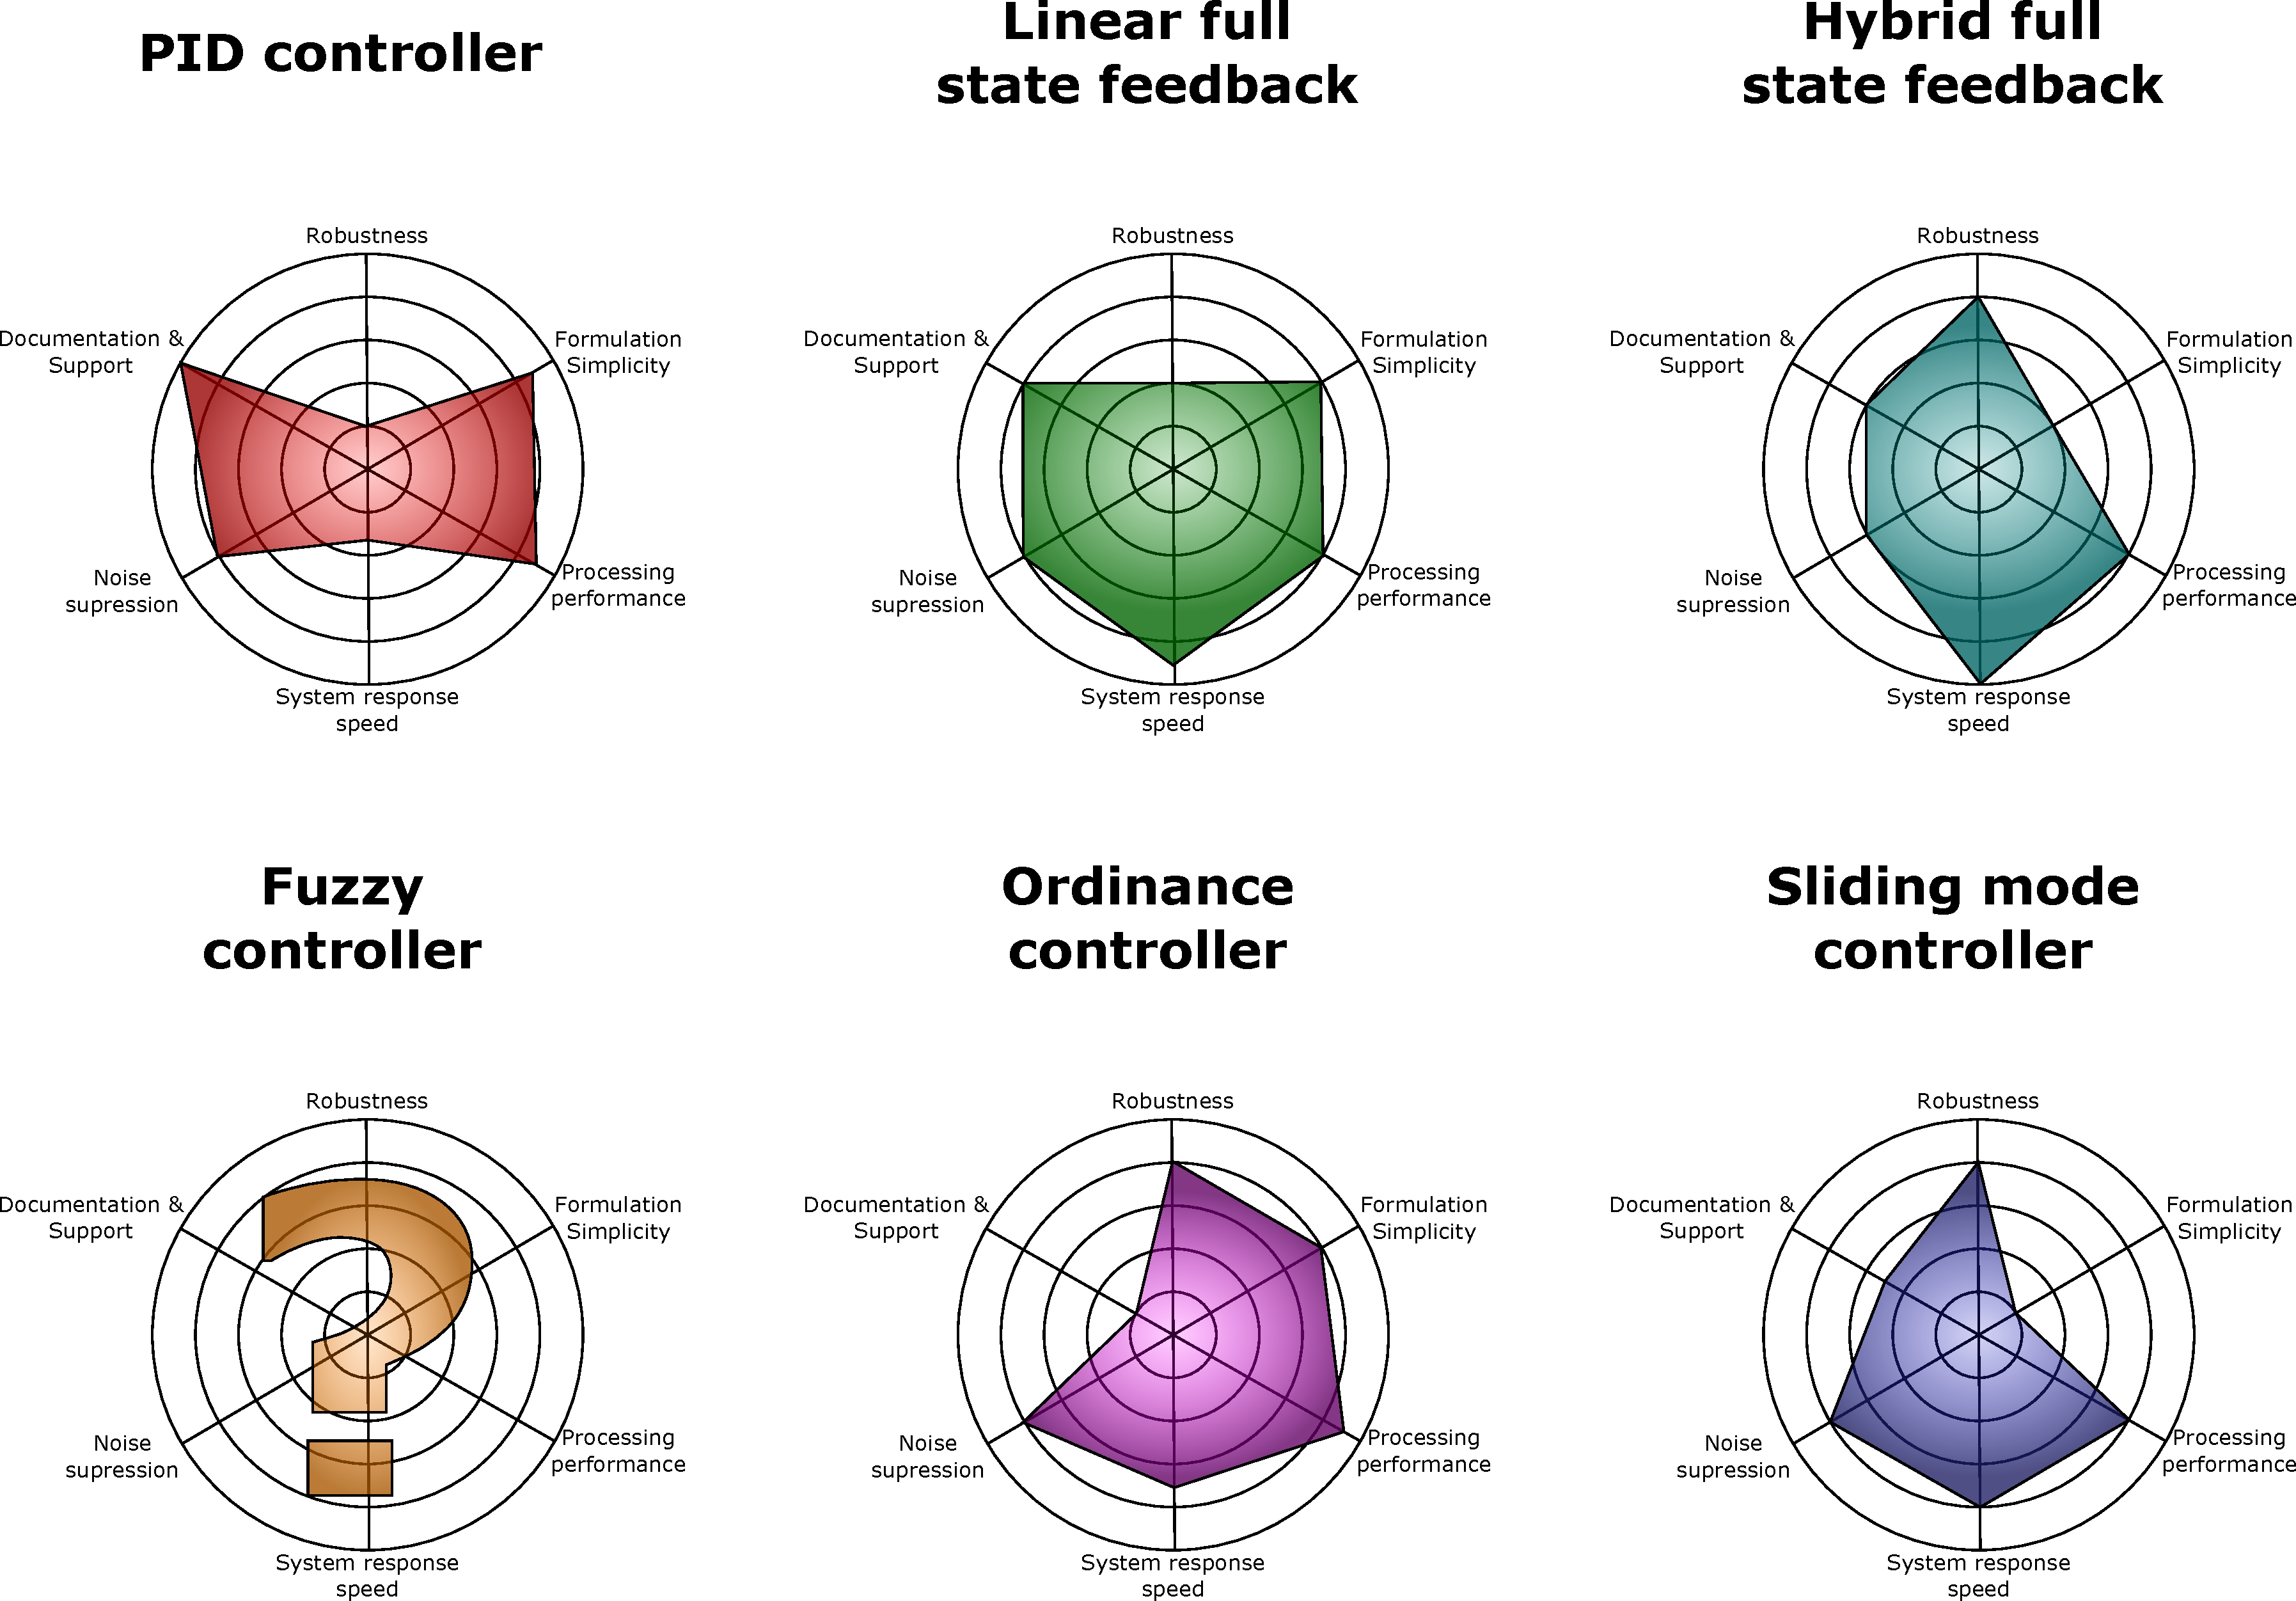
\includegraphics[width=1\textwidth]{img2/ControlCompare}
	\caption{The physical layout of the system}
	\label{fig:PhysicalLayout}
\end{figure}

Final results can’t be concluded yet, because the evaluation of the Fuzzy controller is missing, and the final system is expected to be much more complex than the current test system. Also extensive research must be made to determine the robustness against noise and limited measurements and outputs.

However, the linear full state feedback controller has proven itself to be superior to the other evaluated control systems, because of it’s simple formulation and quality system respone. However, the reliability of the Linear state-feedback controller quickly decreases as the system nonlinearities and uncertanties increase.
In that case the use of a sliding mode controller or ordinance controller is justified, depending on the complexity of the system. The ordinance controller might provide quick and effective results, but if an unambiguous priority can’t be established, then the formulation of a comprehensive sliding mode controller is necessary.